\documentclass[conference,onecolumn]{IEEEtran}
\IEEEoverridecommandlockouts
% The preceding line is only needed to identify funding in the first footnote. If that is unneeded, please comment it out.
\usepackage{cite}
\usepackage{amsmath,amssymb,amsfonts}
\usepackage{graphicx}
\usepackage{subcaption}
\usepackage{textcomp}
\usepackage{xcolor}
\usepackage{float}
\usepackage{algorithm}
% \usepackage{algorithmicx}
\usepackage{advdate}
\usepackage{algpseudocode}
\def\BibTeX{{\rm B\kern-.05em{\sc i\kern-.025em b}\kern-.08em
    T\kern-.1667em\lower.7ex\hbox{E}\kern-.125emX}}
\begin{document}

\title{Comparision and Analysis of Kalman Filter and \\ Particle Filter in Robot Localization \\

\author{
\IEEEauthorblockN{Jiayi Pan*}
\IEEEauthorblockA{\textit{EECS Department} \\
\textit{University of Michigan}\\
Ann Arbor, United States \\
jiayipan@umich.edu}
\and
\IEEEauthorblockN{Changyuan Qiu* \thanks{*Equal Contributions.}}
\IEEEauthorblockA{\textit{EECS Department} \\
\textit{University of Michigan}\\
Ann Arbor, United States \\
peterqiu@umich.edu}



}\\
% {\footnotesize \textsuperscript{*}Note: Sub-titles are not captured in Xplore and
% should not be used}

{\normalsize Project Report, EECS 498 Introduction to Algorithmic Robotics, Fall 2021}\\
{\normalsize Instructor: Dmitry Berenson, Graduate Student Instructor: Tianyi Li}\\
{\normalsize {\AdvanceDate[-1]\today} }
}
\maketitle
% \begin{abstract}

% \end{abstract}



\section{Introduction}


Robot localization is the problem of estimating a robot’s pose relative to a map of its environment \cite{DBLP:books/sp/01/FoxTBD01, DBLP:journals/trob/BetkeG97}.
Applications of robot localization span the whole field of autonomous robotics. This problem is essential for autonomous robotics as a robot will not be able to execute commands and accomplish tasks successfully if it can not determine its current pose accurately, and it has been referred to as “the most fundamental problem to providing a mobile robot with autonomous capabilities” in \cite{DBLP:journals/trob/Cox91}. 


In an unstructured real-world environment, when a robot executes an action, its actual pose will be different from the target pose due to the inevitable motion noise. Moreover, sensor noises add more uncertainties to the problem, making accurate localization even harder. 

In this project, we introduced, compared and analyzed two canonical robot localization algorithms: Kalman Filter and Particle Filter \cite{welch1995introduction, stepanov2011kalman, del1997nonlinear}. In the scenario of a PR2 robot navigating in our designed environment with obstacles following a specific path, we implemented Kalman Filter and Particle Filter for localization. Based on simulation experiments results in Pybullet \cite{coumans2021},  we made a fair comparison of strengths and weaknesses of the two methods. 

\begin{IEEEkeywords}
\centering
Robot Localization, Kalman Filter, Particle Filter
\end{IEEEkeywords}


\section{Approach \& Implementation}

\subsection{Step by Step Quasi-static Motion Model}
In this paper, we use the step by step quasi-static 2D motion to model the motion of the mobile robot.
In this motion model, the robot moves step by step in a quasi-static manner, so that its velocity and acceleration converge to 0.

The state of robot $s$ therefore can be represented only by its current position
\begin{equation}
    \mu = \begin{bmatrix} 
    x \\
    y
    \end{bmatrix}
\end{equation}

And the action (step) $a$ as
\begin{equation}
    u = \begin{bmatrix} 
    \Delta x \\
    \Delta y
    \end{bmatrix}
\end{equation}

However, due to the existence of noise, after the robot takes an action towards the target, the resulting state is disturbed and the robot can only reach somewhere near the target, which we model as 

\begin{equation}
    \mu_{t+1} = A \times \mu_t + B \times u_t + n
\end{equation}

where A is the state-transition model matrix
\begin{equation}
    A = \begin{bmatrix} 
    1 & 0 \\
    0 & 1
    \end{bmatrix}
\end{equation}

B is the control-input model matrix
\begin{equation}
    B = \begin{bmatrix} 
    1 & 0 \\
    0 & 1
    \end{bmatrix}
\end{equation}

n follows the multivariate normal (Gaussian) distribution with process noise covariance matrix $R$
\begin{equation}
    n \sim \mathcal{N}\left(0, R\right)
\end{equation}

\subsection{Sensor Model with Gaussian Noise}
Mobile robots are usually equipped with various sensors, like GPS, camera, microphone, LiDar to constantly update their knowledge about the surrounding environment.

In this setup, for the localization purpose, we consider the GPS sensor with input $z$ representing its sensed position
\begin{equation}
    z = \begin{bmatrix} 
    x \\
    y
    \end{bmatrix} + n'
\end{equation}

It is noteworthy that due to the existence of noise, the sensed position $z$ is not accurate. As Kalman filter relies on the assumption that errors obey normal (Gaussian) distribution, we model the noise $n'$ accordingly

\begin{equation}
    n \sim \mathcal{N}\left(0, Q\right)
\end{equation}
where $Q$ it its covariance matrix (also called Kalman gain under the setup of Kalman filter).




\subsection{Kalman Filter}


A general picture of the Kalman Filter method is illustrated in Algorithm 1, with detailed procedures and implementations of Kalman Filter illustrated in Algorithm 2.

\begin{algorithm}[H]
\caption{Kalman Filter Method}\label{alg:kfm}
\textbf{Input:} Gaussian of robot's initial state $(\mu_0,\Sigma_0)$
\begin{algorithmic}
        \While {Robot takes action $u_t$ at time t}
        \State get sensor input $z_t$
        \State estimate Gaussian of robot's state $(\mu_t,\Sigma_t) = \text{Kalman Filter}(\mu_{t-1},\Sigma{t-1}, u_t, z_t)$ 
        \EndWhile
\end{algorithmic}
\end{algorithm}
% A detailed procedures and implementations of Kalman Filter is illustrated in Algorithm 2.

\begin{algorithm}[H]
\caption{Kalman Filter}\label{alg:kf}
\textbf{Input:} Gaussian of the estimated current state ($\mu_{t-1}$, $\Sigma_{t-1}$), action $u_{t}$, sensor input $z_{t}$\\
\textbf{Set:} state-transition model matrix $A$, control-input model matrix $B$,  observation model matrix $C$, process noise matrix $R$, Kalman gain matrix $Q$
\begin{algorithmic}
      \State $\bar{\mu_t} \gets A \mu_{t-1} + B u_t$ \Comment{Prediction}
      \State $\bar{\Sigma_t} \gets A \Sigma_{t-1} A^T + R$

      \State $K_t = \bar{\Sigma_t} C^T (C \bar{\Sigma_t} C^T + Q)^{-1}$ \Comment{Correction}
      \State $\mu_t = \bar{\mu_t} + K_t(z_t - C \bar{\mu_t})$
      \State $\Sigma_t = (I - K_t C)\bar{\Sigma_t}$
\end{algorithmic}
\textbf{Output:} Gaussian of estimated next state ($\mu_{t}$, $\Sigma_{t}$),
\end{algorithm}

\subsection{Particle Filter}

A general picture of the Particle Filter method is illustrated in Algorithm 3, with detailed procedures and implementations of Particle Filter method illustrated in Algorithm 4.


\begin{algorithm}[H]
\caption{Particle Filter Method}\label{alg:pfm}
\textbf{Input:} Number of particles $M$, particles initial distributions $P$ with weigts $W$
\begin{algorithmic}
        \While {Robot takes action $u_t$ at time t}
        \State get sensor input $z_t$
        \State update particles and weights $(P, W) = \text{Particle Filter}(P, W, M, u_t, z_t)$
        \EndWhile
\end{algorithmic}
\end{algorithm}


\begin{algorithm}[H]
\caption{Particle Filter}\label{alg:pf}
\textbf{Input:} particles from previous state $P$ with weights $W$, number of particles  $M$, action $u_{t}$, sensor input $z_{t}$ \\
\textbf{Set:} state-transition model matrix $A$, control-input model matrix  $B$, covariance matrix for sampling $\Sigma$, function to check if a particle is in reachable region $IsReachable(\cdot)$

\begin{algorithmic}
      \For{particle $p$ in $P$} \Comment{Update and sample particles (Propagate)}
      \State $p' = A \times p+B \times u_t$  
      \State sample new particle $p'_s$ from distribution $N(p',\Sigma)$
        \While{not $IsReachable(p'_s)$}
      \State re-sample a new particle $p'_s$ from distribution $N(p',\Sigma)$
        \EndWhile
        \State $p = p'_s$
      \EndFor
      \For{$m = 1$ to $M$} \Comment{Update Weight}
    %   TODO: correct it
    %   \State $W[m] = \frac{1}{|{z_t - P[m]}|}$
      \State $W[m] = \operatorname{det}(2 \pi \mathbf{\Sigma})^{-\frac{1}{2}} e^{-\frac{1}{2}(z_t - P[m])^{\top} \boldsymbol{\Sigma}^{-1}(z_t - P[m])}$
      \EndFor
      \State Construct empty particle list $P'$  \Comment{Resample}
      \For{$m = 1$ to $M$}
      \State draw $i$ with probability $\propto W[i]$
      \State add $P[i]$ from $P$ to $P'$
      \EndFor
      \State $P = P'$
\end{algorithmic}
\textbf{Output:} updated particles $P$ with weights $W$
\end{algorithm}



\section{Experiments \& Results}

\subsection{Experiment Setup}

In order to make a fair comparison between Kalman Filter and Particle Filter under different circumstances, we designed the environments as well as robot's execution path. An overview of the environment as well as the robot's execution path is illustrated in Figure \ref{fig: maze}.


    
    



\begin{figure}[H] 
 \centering 
 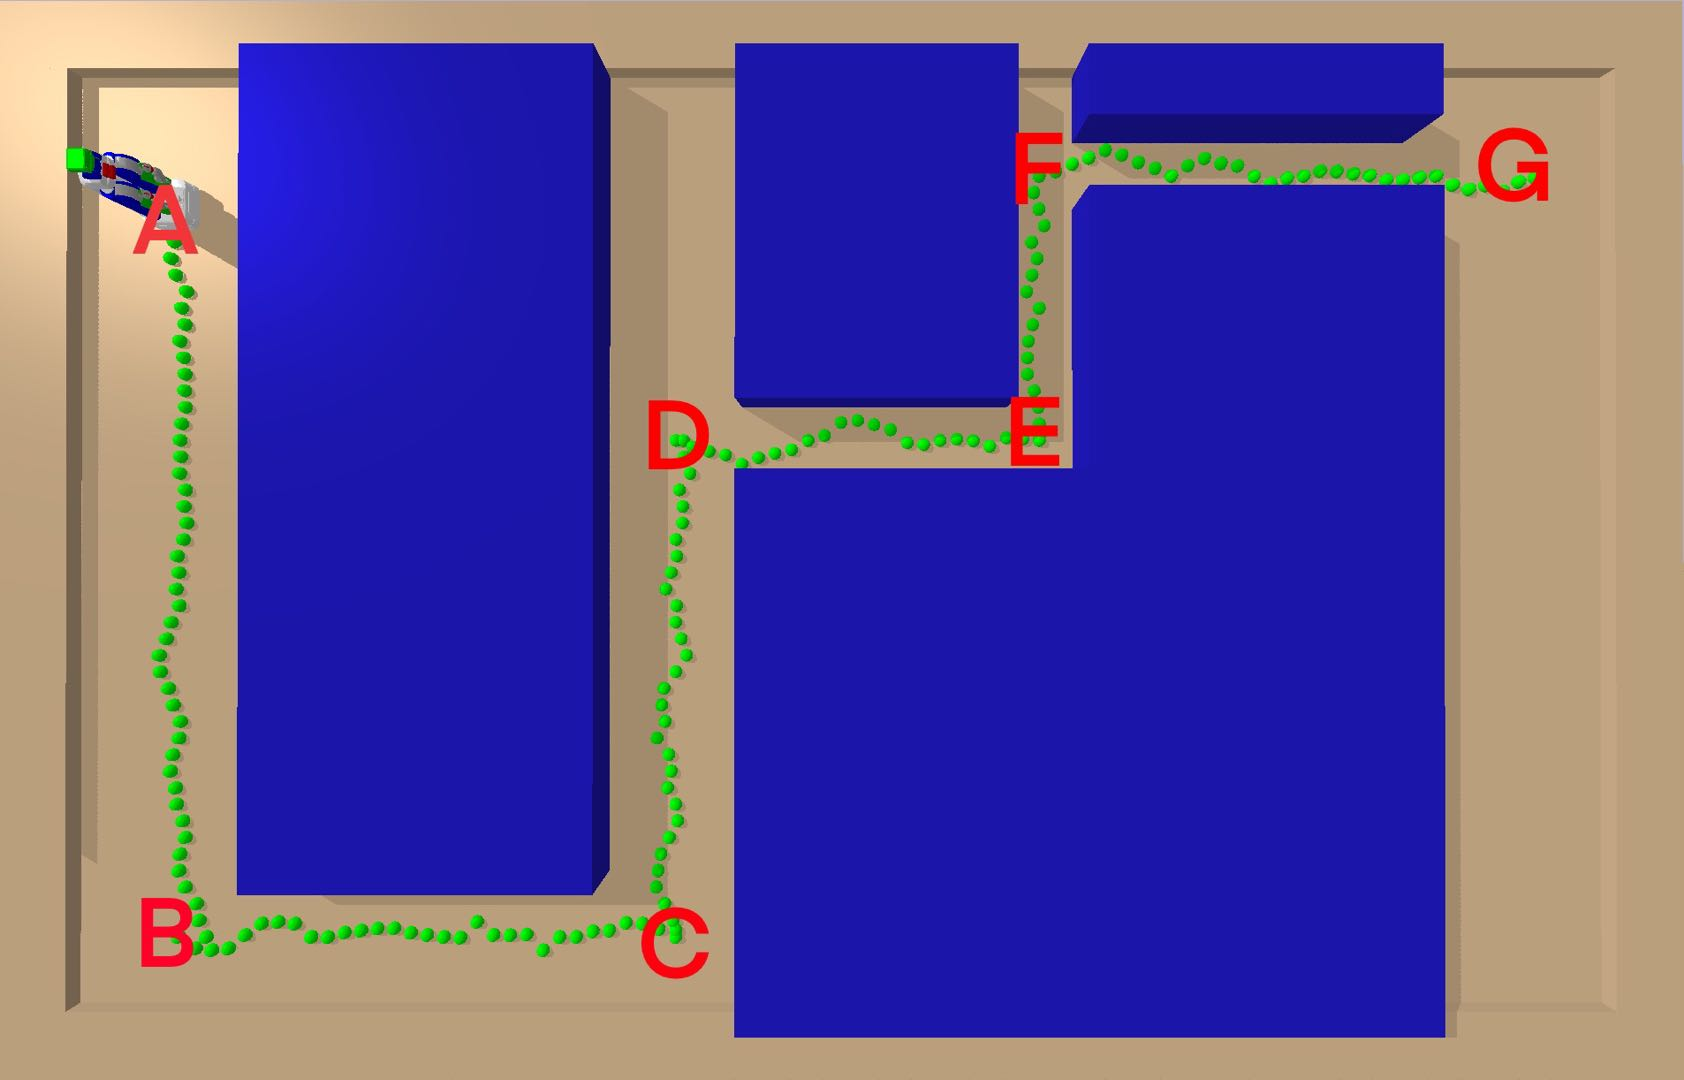
\includegraphics[width=0.53\textwidth]{Figs/Maze.jpg} 
 \caption{An Overview of the map "Maze" and robot's execution path} 
 \label{fig: maze} 
 \end{figure}

More specifically, we divide the path into 3 sub-paths:

\begin{itemize}
    \item Path A-B. Where the path is most spacious and flat and the robot will not have any collisions with the walls.
    
    

   \item Path B-C-D. Where the path becomes narrower and based on the motion noise the robot might have some collisions with the walls.
   
   
    \item Path D-E-F-G. Where the path is the narrowest and the robot is expected to have a lot of collisions with the walls.
    \end{itemize}

\subsection{Result}
%% THE BIG TABLE OF RESULTS!
Comprehensive experiments were conducted under this simulation environment. 





\begin{figure}[H]
  \centering
  Result of Kalman Filter
  \medskip

  \begin{subfigure}[t]{.3\linewidth}
    \centering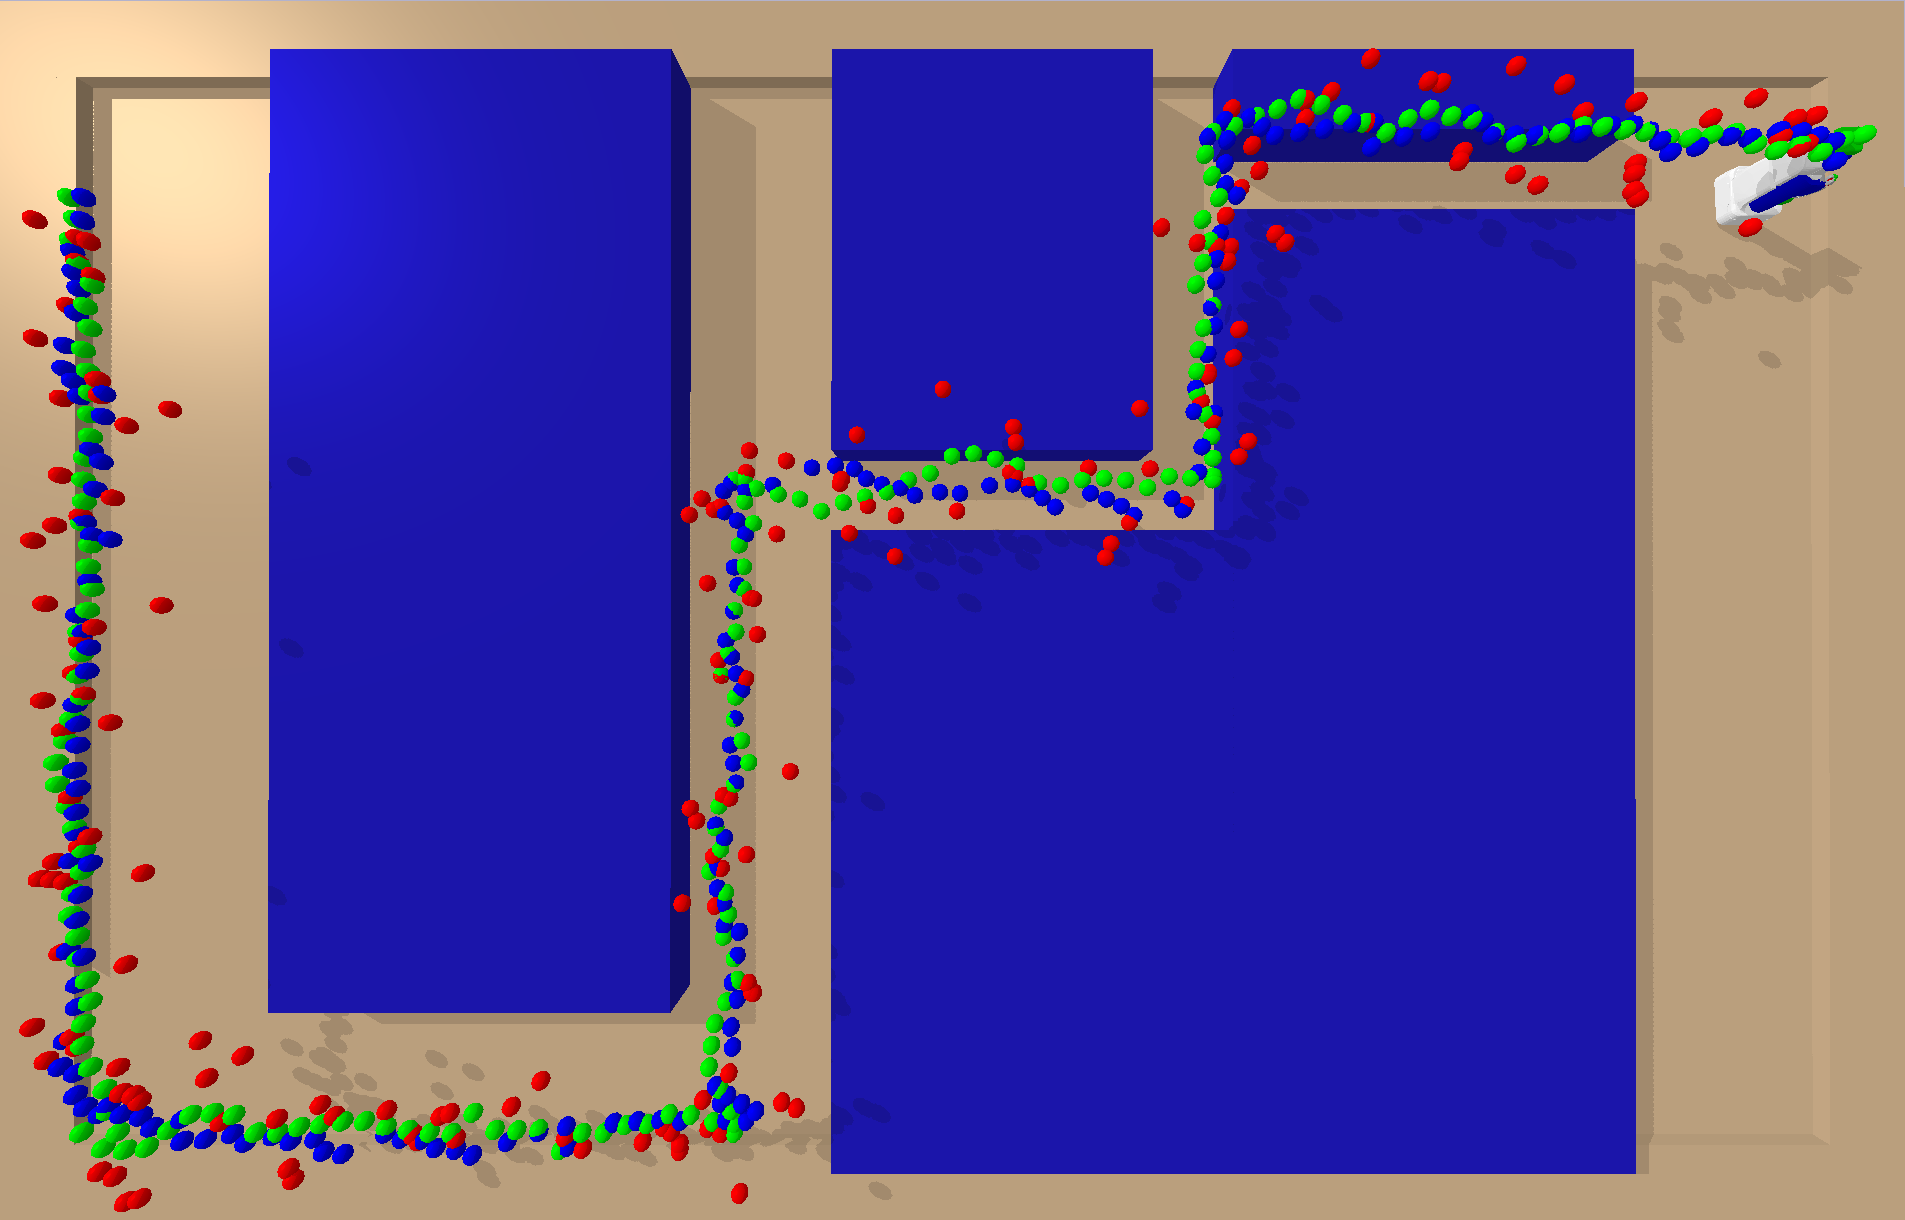
\includegraphics[width=\linewidth]{Figs/Kalman.png}
    \caption{PyBullet Simulation}
  \end{subfigure}
  \begin{subfigure}[t]{.3\linewidth}
    \centering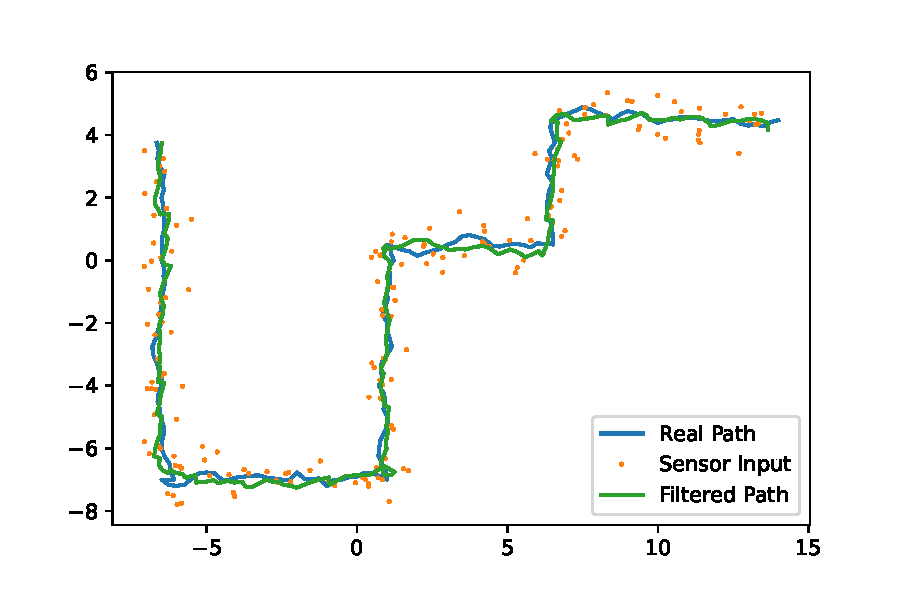
\includegraphics[width=\linewidth]{Figs/Kalman FilterPath.pdf}
    \caption{Real Path, Sensor Input, Filter Result}
  \end{subfigure}
  \begin{subfigure}[t]{.3\linewidth}
    \centering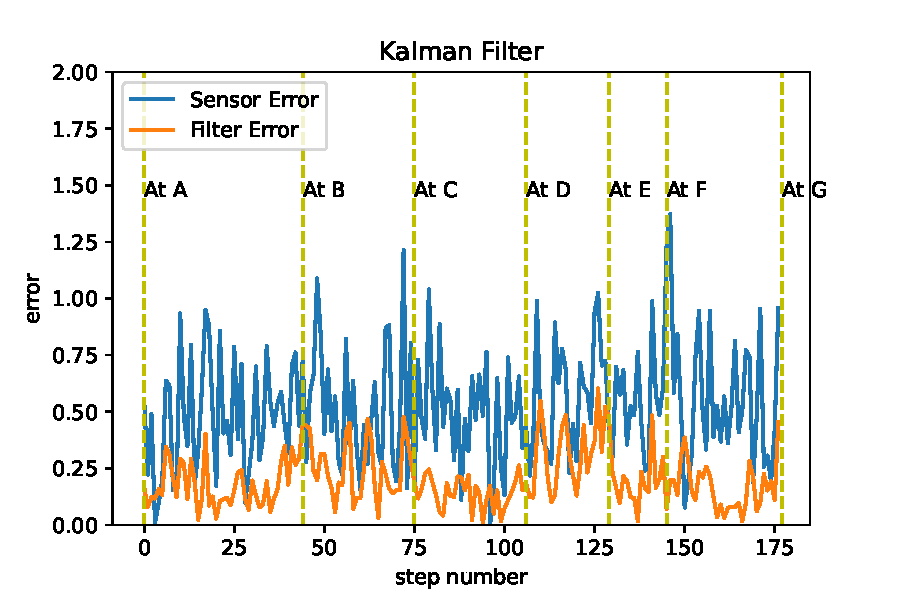
\includegraphics[width=\linewidth]{Figs/Kalman FilterError.pdf}
    \caption{Error after/before filtering}
  \end{subfigure}

   \smallskip\hrulefill \smallskip
  
  
  Result of Particle Filter with 10 Particles
  \medskip

  \begin{subfigure}[t]{.3\linewidth}
    \centering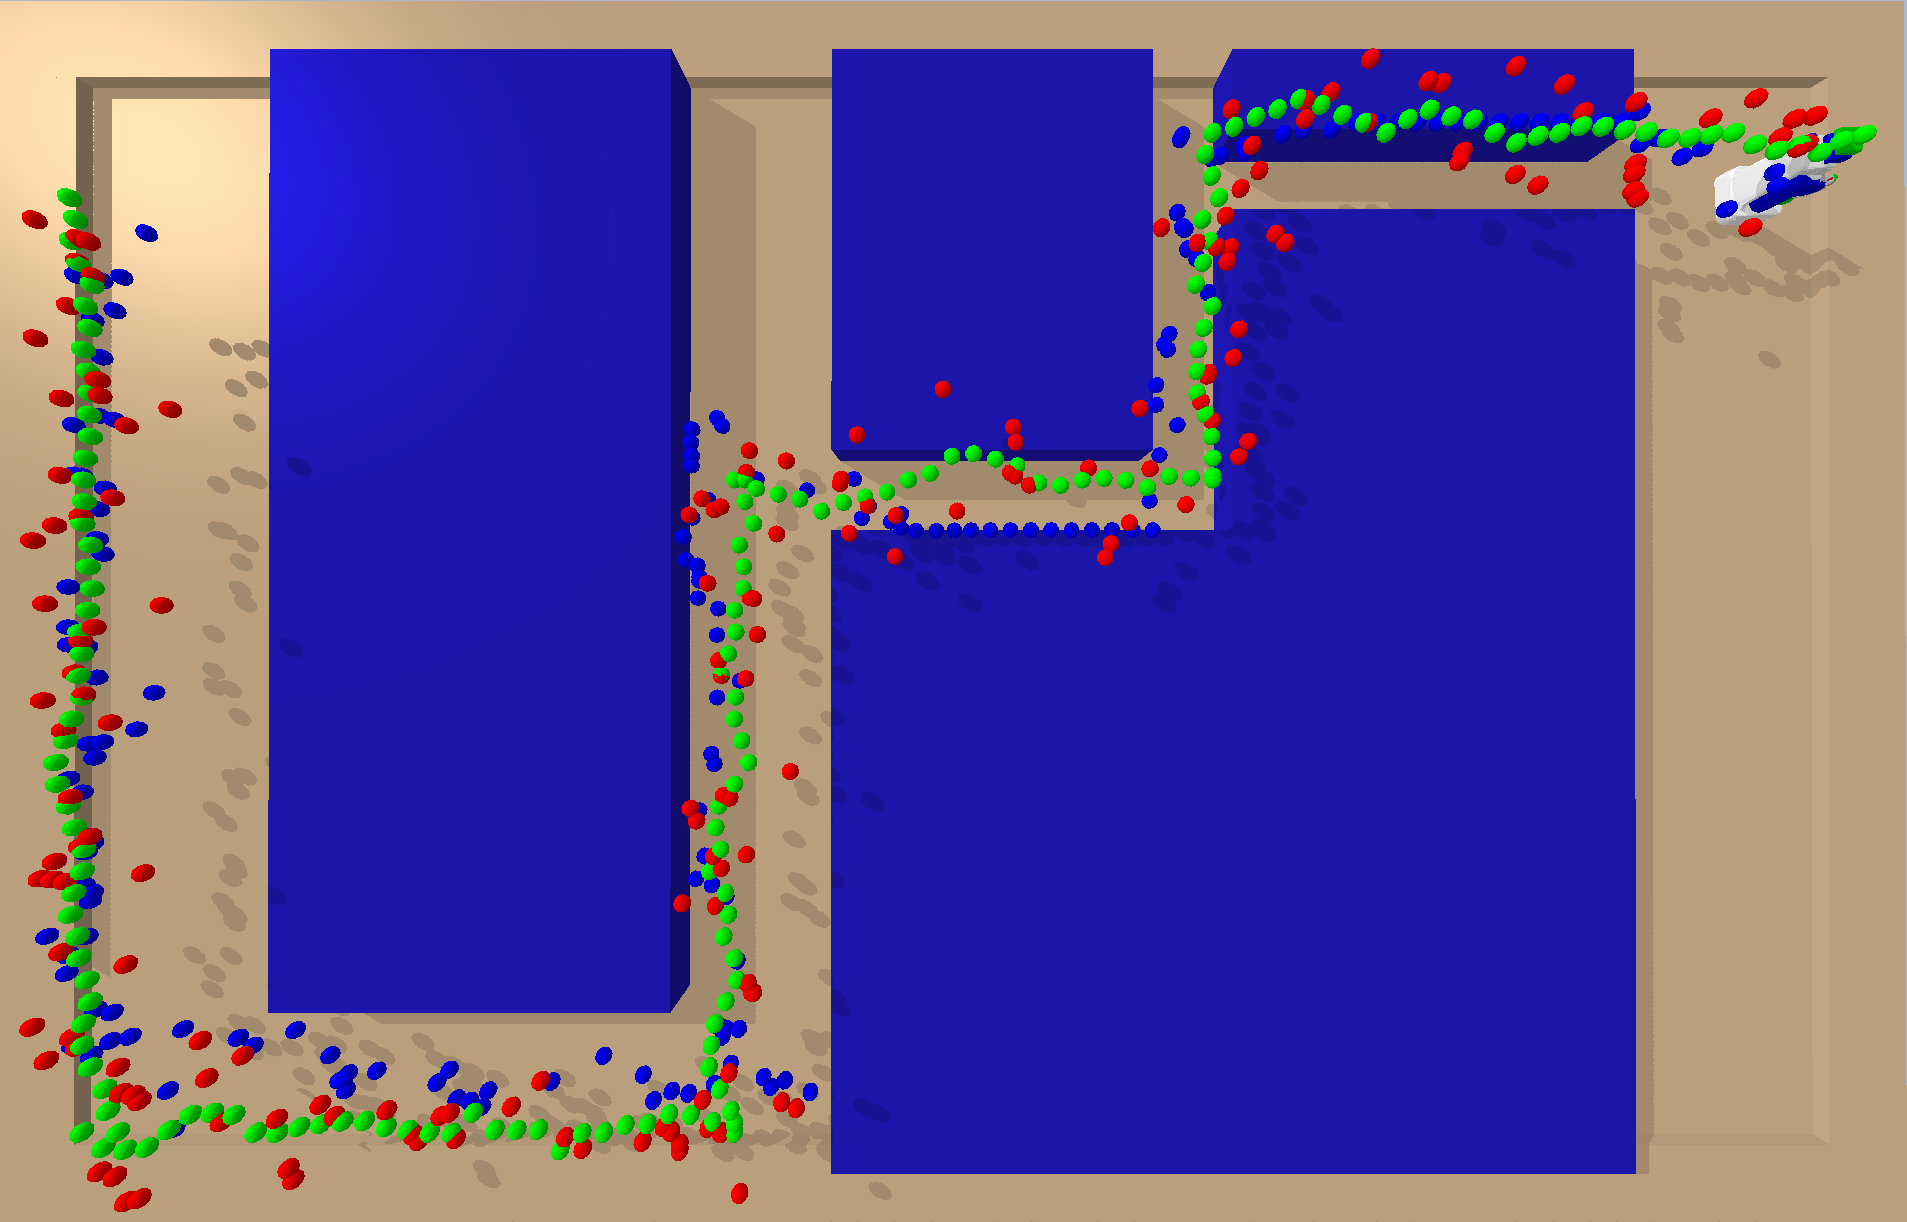
\includegraphics[width=\linewidth]{Figs/p10.png}
    \caption{PyBullet Simulation}
  \end{subfigure}
  \begin{subfigure}[t]{.3\linewidth}
    \centering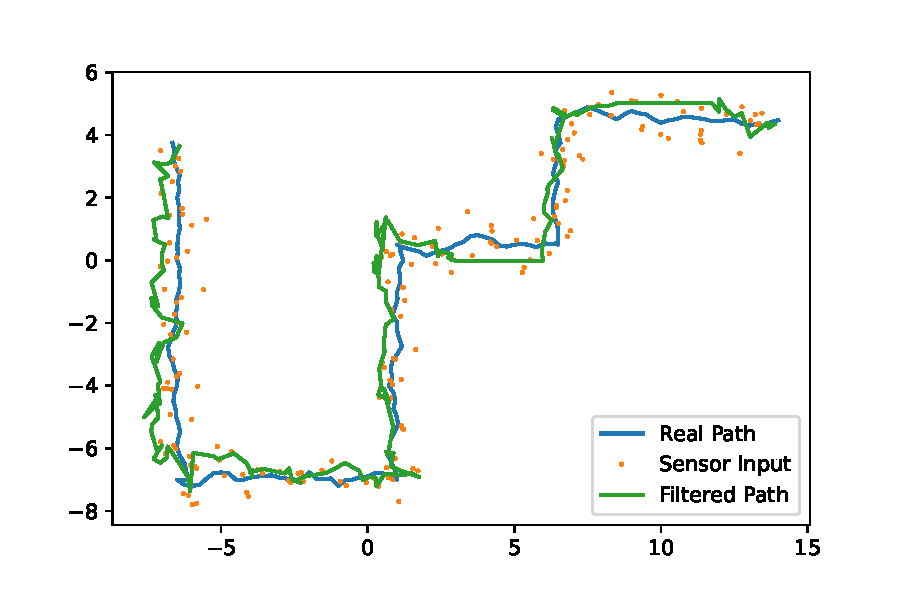
\includegraphics[width=\linewidth]{Figs/Particle Filter + 10Path.pdf}
    \caption{Real Path, Sensor Input, Filter Result}
  \end{subfigure}
  \begin{subfigure}[t]{.3\linewidth}
    \centering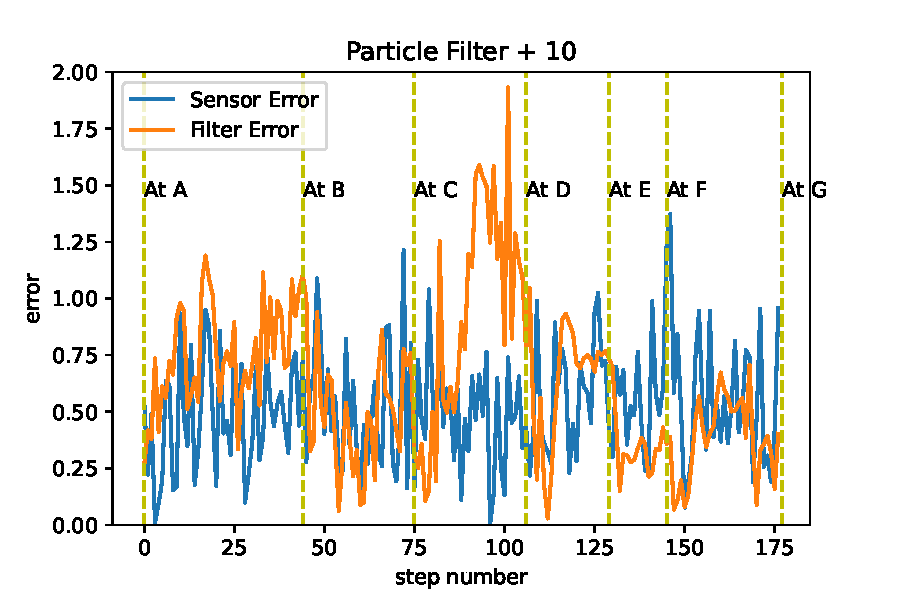
\includegraphics[width=\linewidth]{Figs/Particle Filter + 10Error.pdf}
    \caption{Error after/before filtering}
  \end{subfigure}
%   \bigskip\hrulefill\bigskip

   \smallskip\hrulefill \smallskip
  
  Result of Particle Filter with 100 Particles
  \medskip

  \begin{subfigure}[t]{.3\linewidth}
    \centering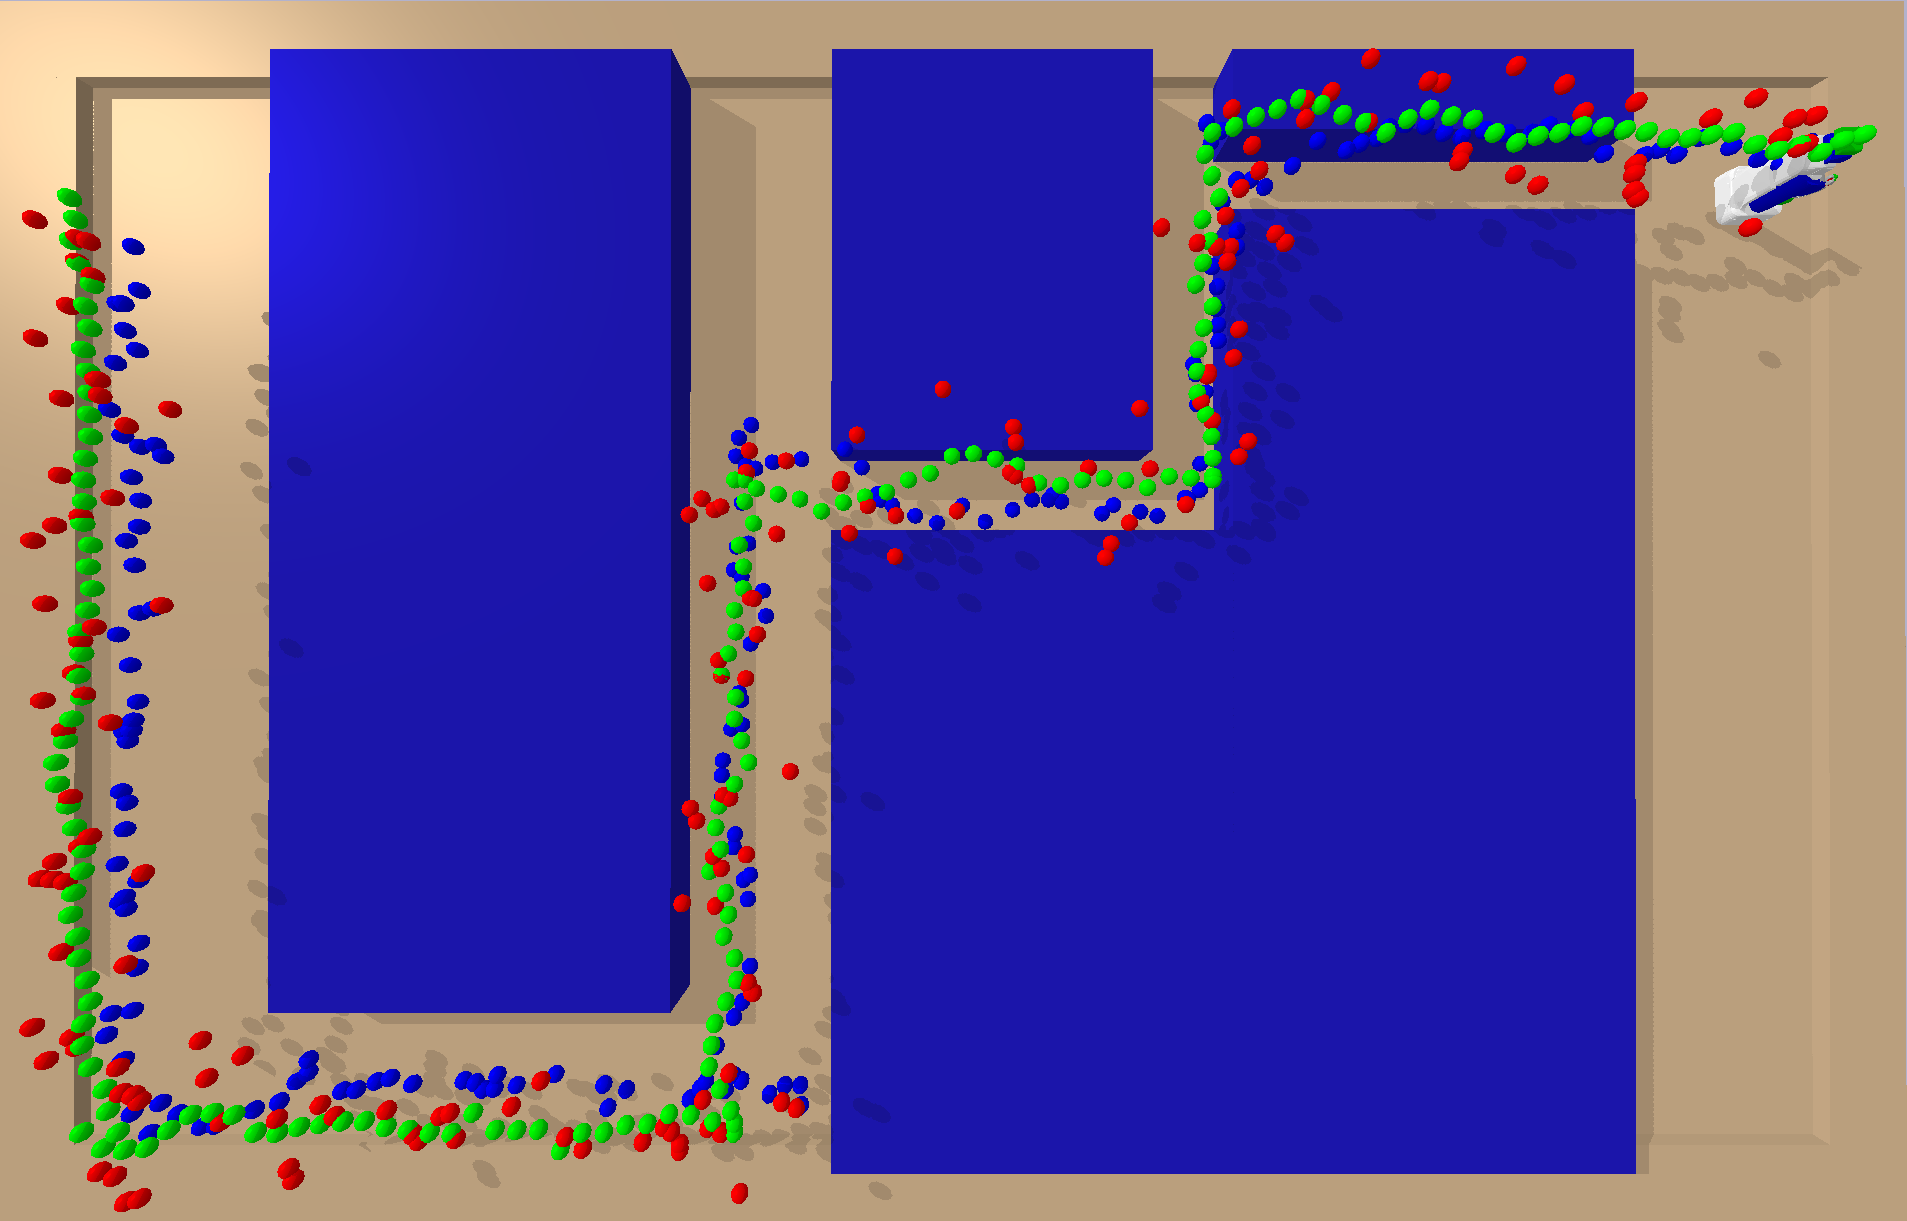
\includegraphics[width=\linewidth]{Figs/p100.png}
    \caption{PyBullet Simulation}
  \end{subfigure}
  \begin{subfigure}[t]{.3\linewidth}
    \centering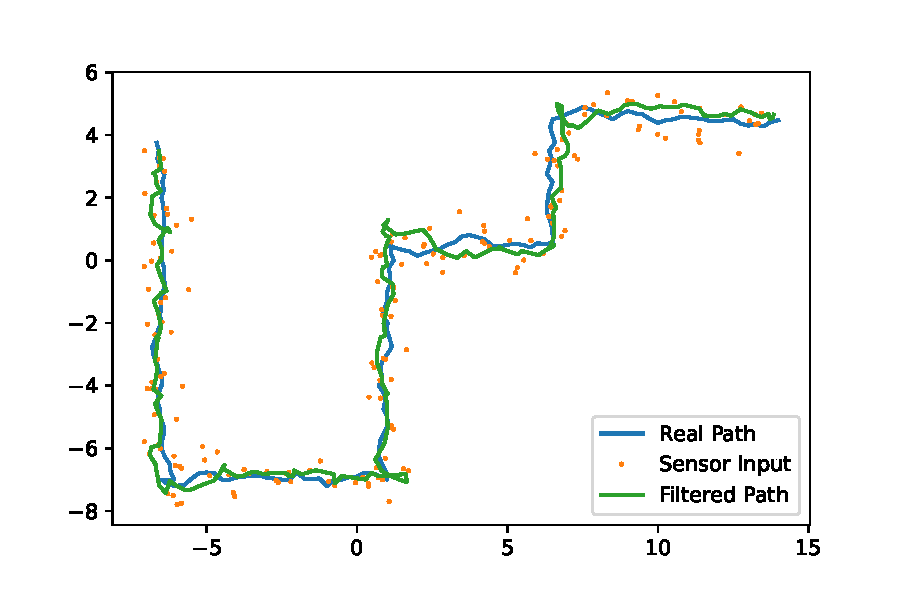
\includegraphics[width=\linewidth]{Figs/Particle Filter + 100Path.pdf}
    \caption{Real Path, Sensor Input, Filter Result}
  \end{subfigure}
  \begin{subfigure}[t]{.3\linewidth}
    \centering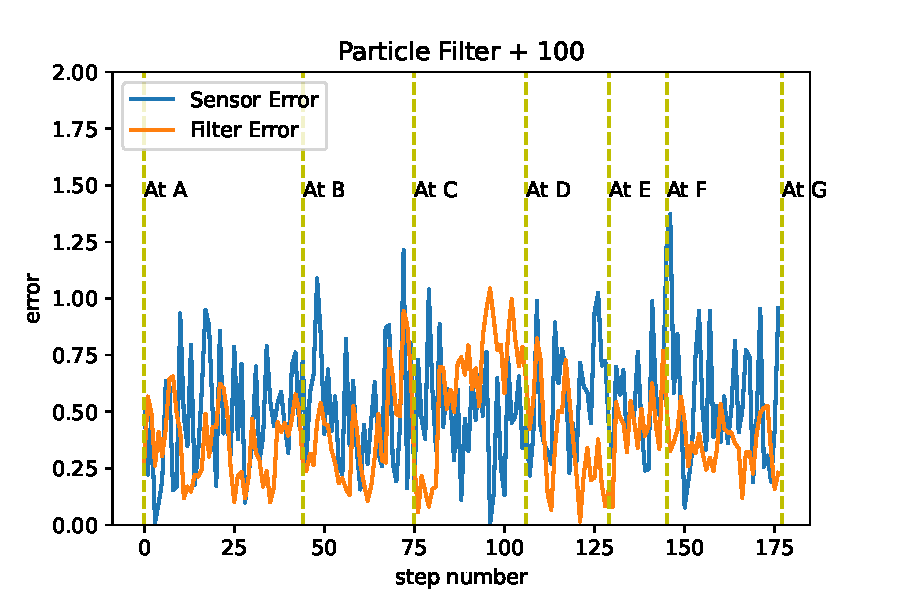
\includegraphics[width=\linewidth]{Figs/Particle Filter + 100Error.pdf}
    \caption{Error after/before filtering}
  \end{subfigure}

%   \bigskip\hrulefill\bigskip
   \smallskip\hrulefill \smallskip
   
  Result of Particle Filter with 1000 Particles
  \medskip

  \begin{subfigure}[t]{.3\linewidth}
    \centering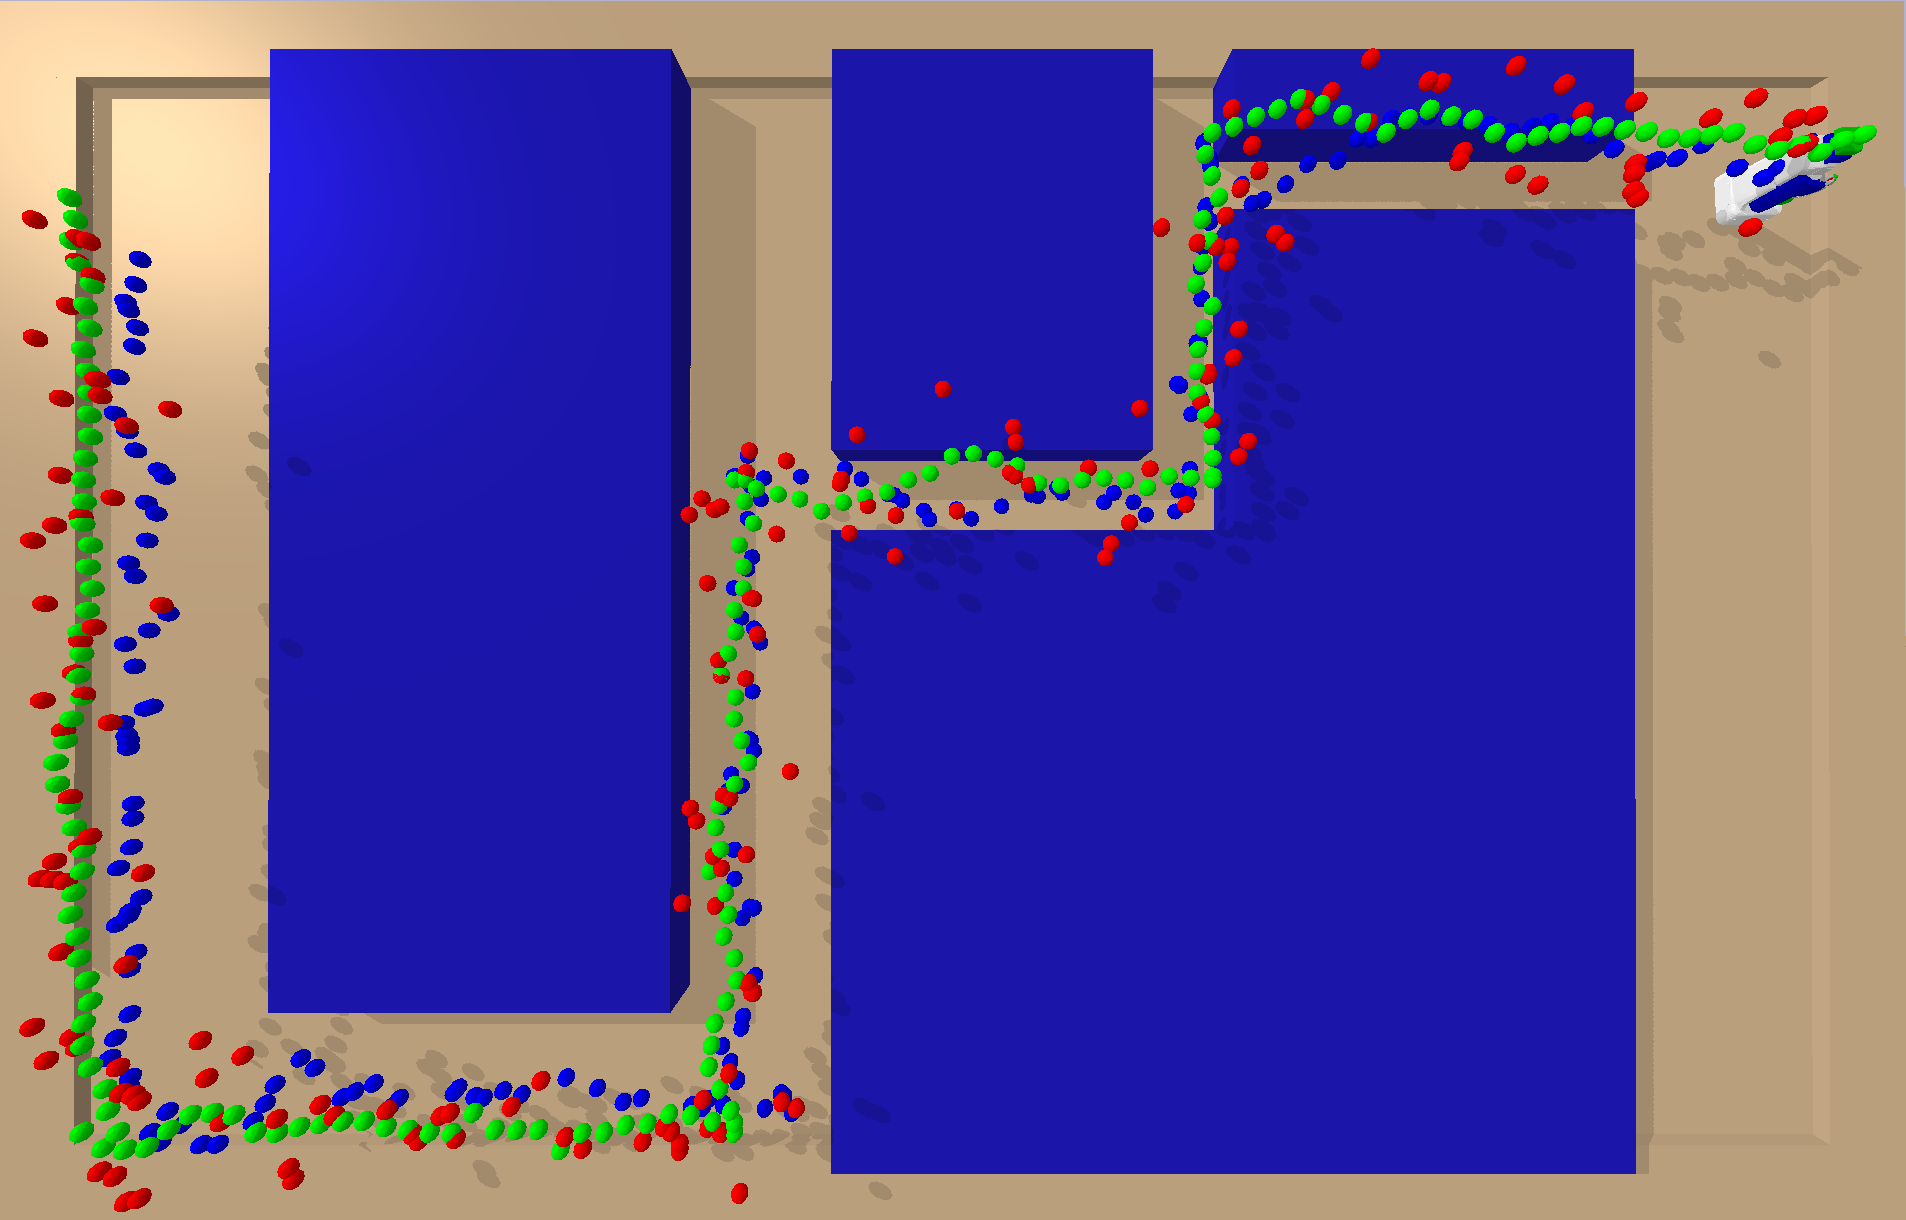
\includegraphics[width=\linewidth]{Figs/p1000.png}
    \caption{PyBullet Simulation}
  \end{subfigure}
  \begin{subfigure}[t]{.3\linewidth}
    \centering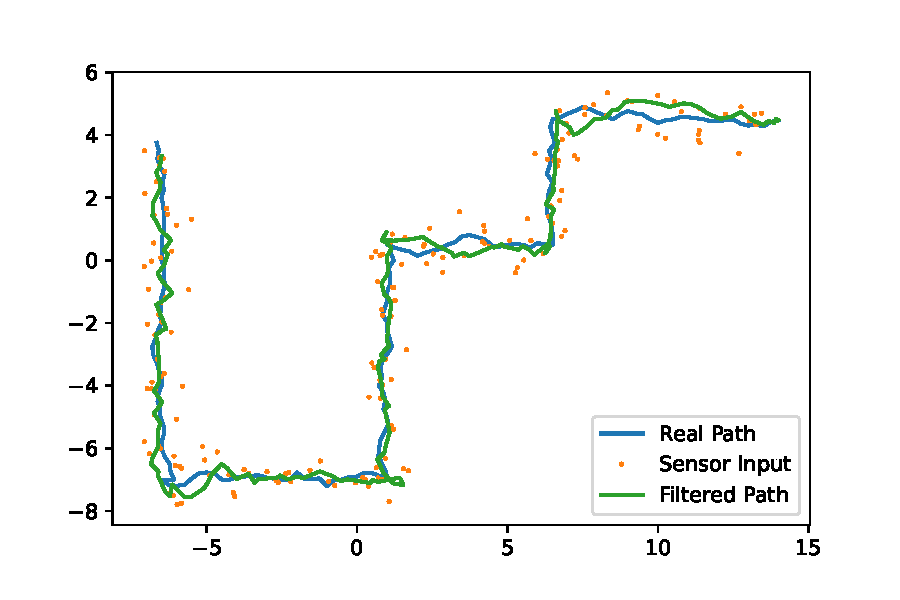
\includegraphics[width=\linewidth]{Figs/Particle Filter + 1000Path.pdf}
    \caption{Real Path, Sensor Input, Filter Result}
  \end{subfigure}
  \begin{subfigure}[t]{.3\linewidth}
    \centering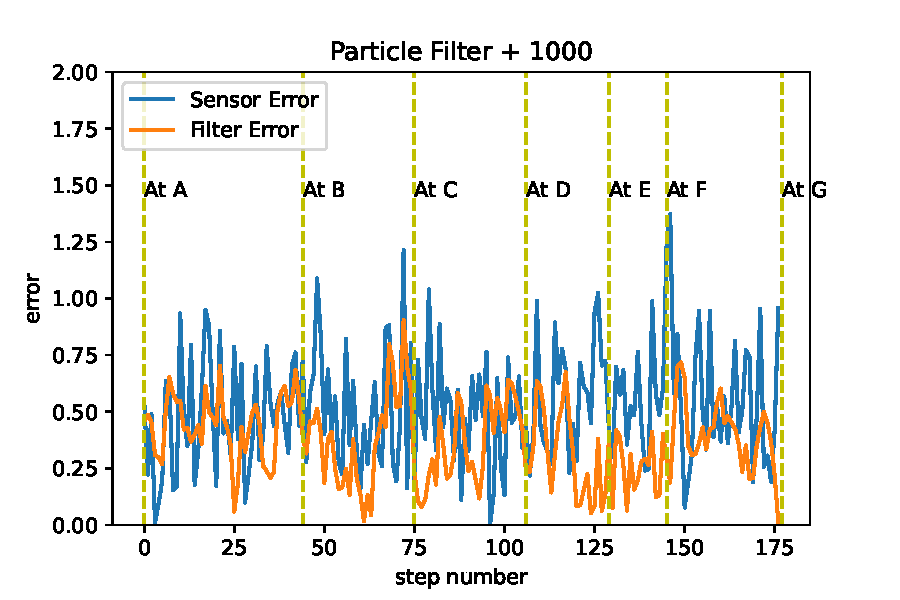
\includegraphics[width=\linewidth]{Figs/Particle Filter + 1000Error.pdf}
    \caption{Error after/before filtering}
  \end{subfigure}

%   \bigskip\hrulefill\bigskip
   \smallskip\hrulefill \smallskip
  
  
  Result of Particle Filter with 10,000 Particles
  \medskip

  \begin{subfigure}[t]{.3\linewidth}
    \centering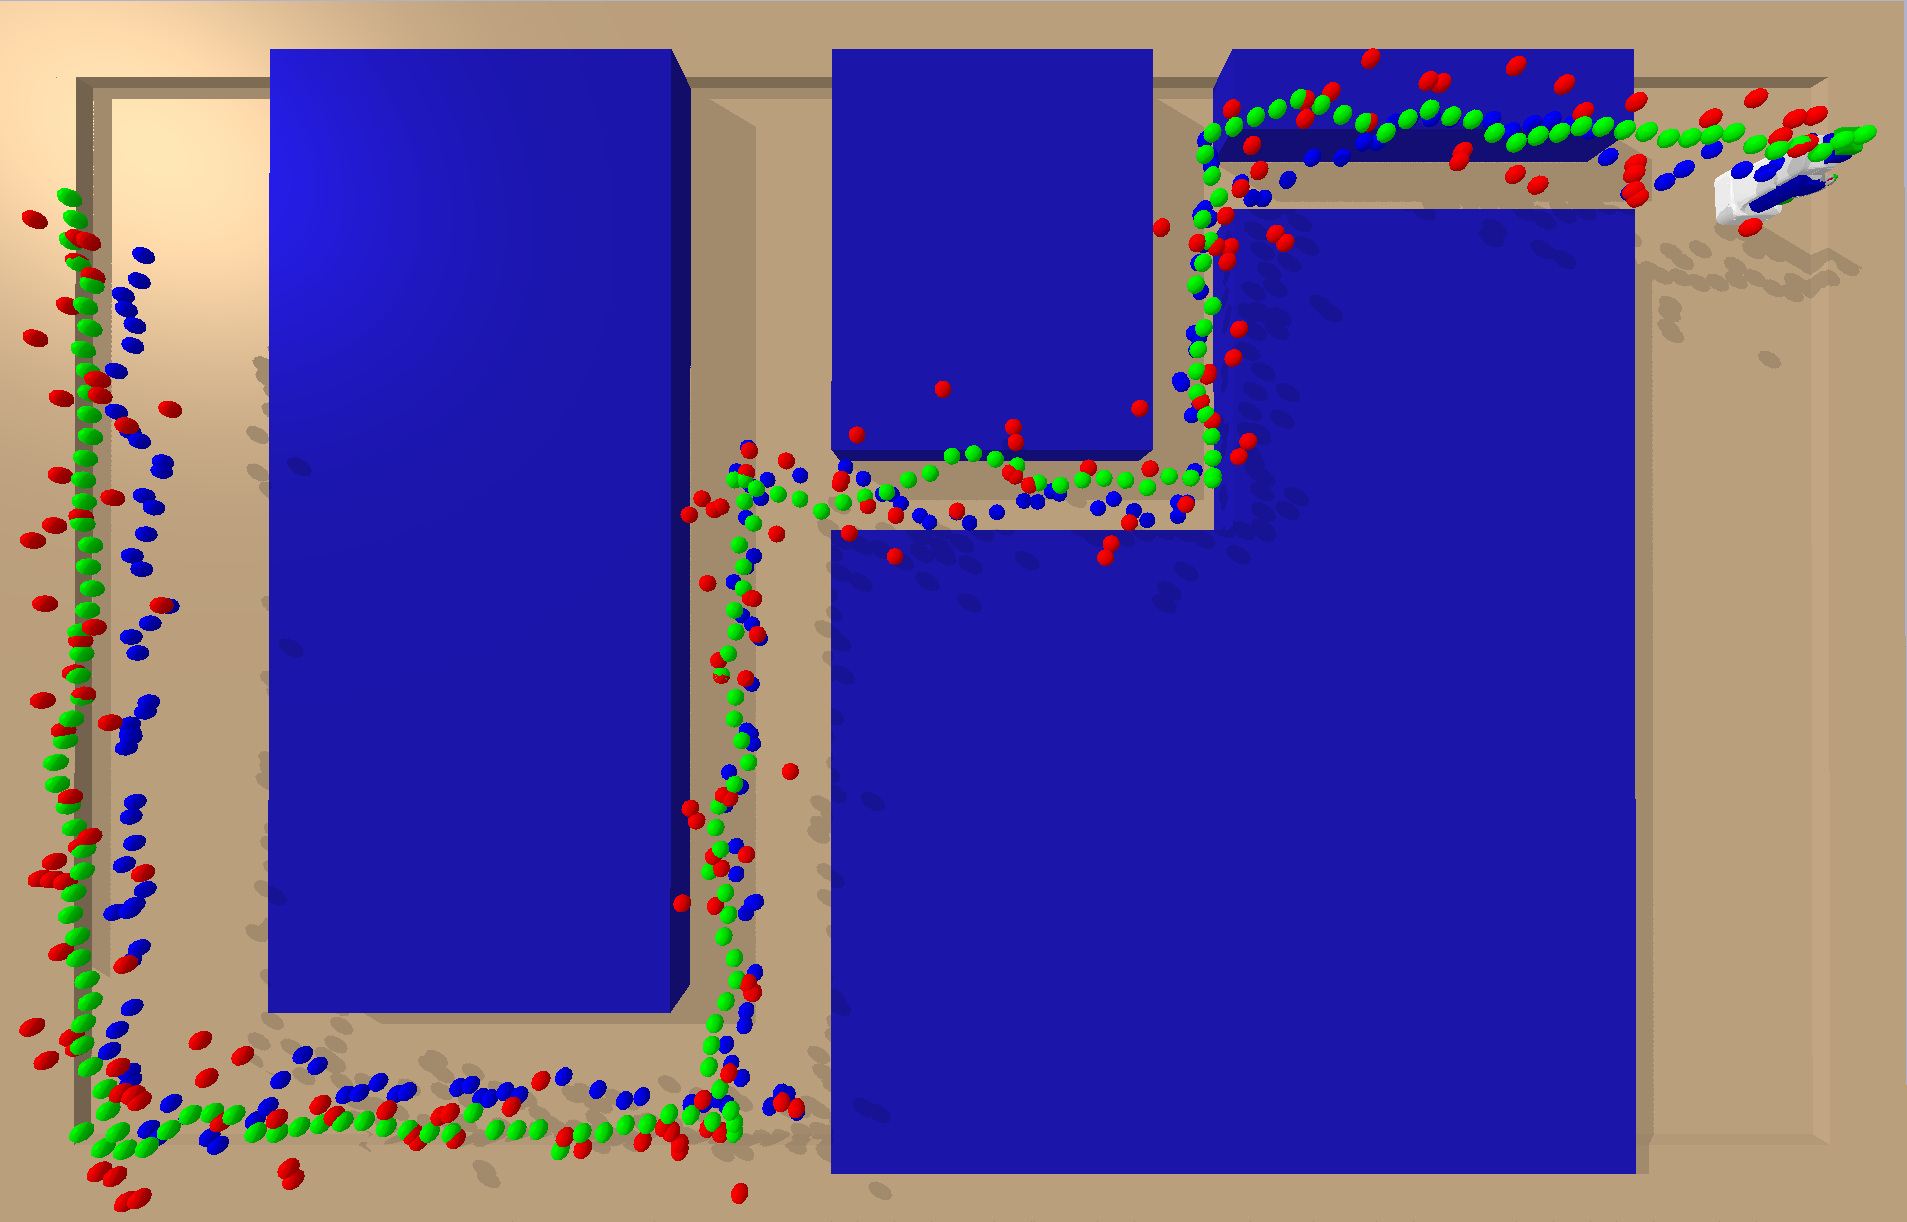
\includegraphics[width=\linewidth]{Figs/p10000.png}
    \caption{PyBullet Simulation}
  \end{subfigure}
  \begin{subfigure}[t]{.3\linewidth}
    \centering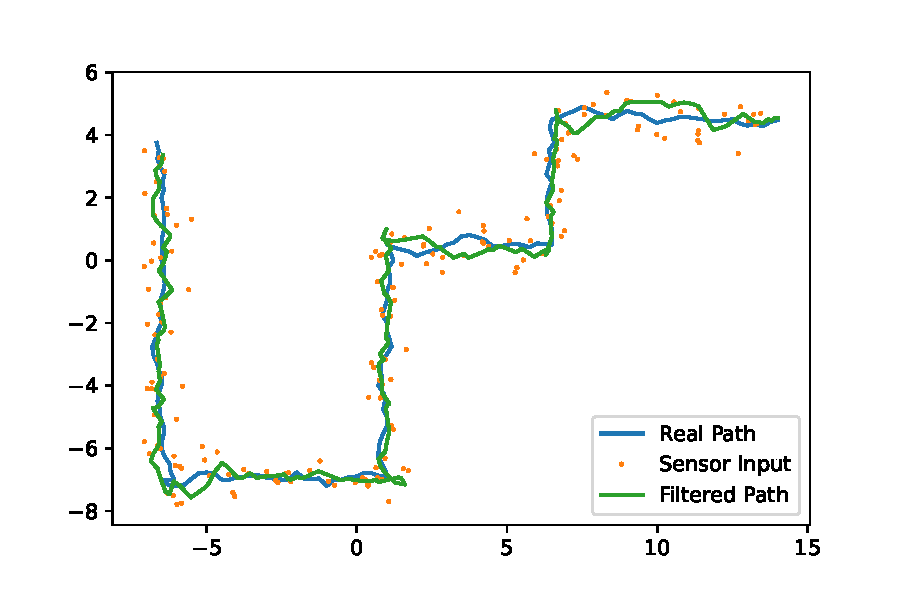
\includegraphics[width=\linewidth]{Figs/Particle Filter + 10000Path.pdf}
    \caption{Real Path, Sensor Input, Filter Result}
  \end{subfigure}
  \begin{subfigure}[t]{.3\linewidth}
    \centering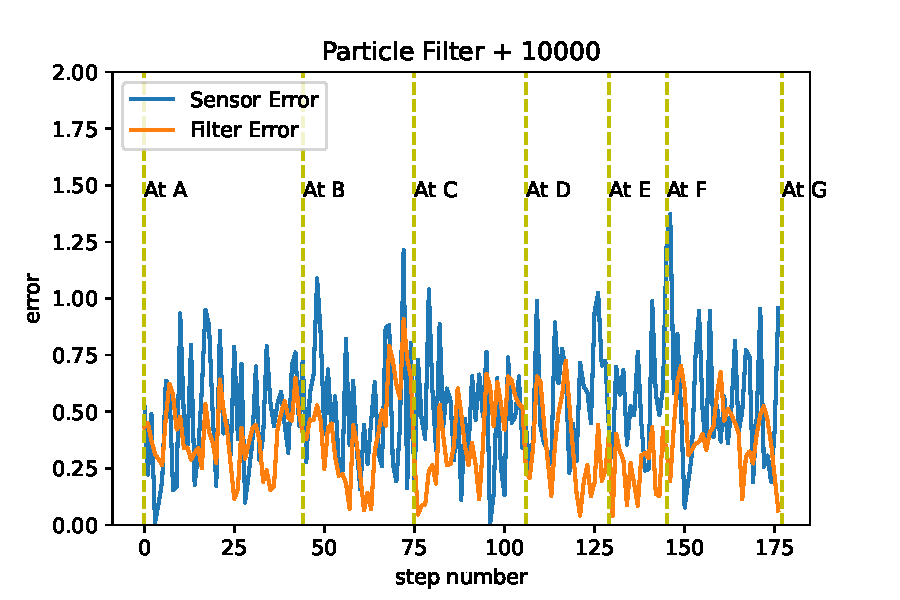
\includegraphics[width=\linewidth]{Figs/Particle Filter + 10000Error.pdf}
    \caption{Error after/before filtering}
  \end{subfigure}
  
%   \bigskip\hrulefill\bigskip
\caption{Experiment Results in Pybullet Simulation}
\label{fig: result}
\end{figure}

We apply Kalman filter and particle filter methods with 10, 100, 1000, 10000 particles respectively in this setup and summarized the result in Figure \ref{fig: result} and Table \ref{tab: stat}.

For ablation study purposes, the sensor noise was generated beforehand and was the same for all methods.

 \begin{table}[H] 
 \centering 
 \begin{tabular}{c|c|c} 
  Method Name & Accumulated Error & Runtime\\ \hline
  Base & - & 16.698s \\
  Kalman Filter &  35.718 &17.176s\\
  Particle Filter with 10 particles& 109.984  &17.721s\\
  Particle Filter with 100 particles&  73.732 &19.542s\\
  Particle Filter with 1000 particles& 66.172 &30.330s\\
  Particle Filter with 10,000 particles&  66.544 &140.861s\\
 \end{tabular}% 
 \caption{Quantitative Experiment Results. Base denotes running the simulation without applying any localization algorithm} 
 \label{tab: stat}% 
 \end{table}% 

\subsection{Discussion \& Conclusion}

\begin{itemize}
    \item Kalman filter is more efficient than Particle Filter.
    
    
    We discovered that Kalman filter is more efficient than particle filter. In our experiment, from Table \ref{tab: stat}, Kalman filter consumes only $24\%$ of time for particle filter with 10 particles and adds little cost to the overall simulation runtime. However, running particle filter with more particles (eg: 1000, 10000) will significantly increasing the simulation time. For particle filter with 10,000 particles, it takes about 790X more time than the Kalman filter. 
    
    The underlying reason is that while Kalman filter uses Gaussian distribution to model the state of robot, particle filter relies on sampling various particles to model it, which is less computationally efficient.
    
   \item Kalman filter has lower overall error under this setup.
   
    We discovered that Kalman filter generally has lower error under this setup. From Table \ref{tab: stat}, we can see that the accumulated error for Kalman filter is lower than any setup of the particle filter, demonstrating the strength of Kalman filter when facing Gaussian noise.
    
    \item Particle filter generates realistic result while Kalman might not.
    
    Though Kalman filter produces lower error overall, we discovered that the output of particle filter is more realistic. From Figure \ref{fig: result}, we can find that though Kalman filter generates satisfactory results during Path A-D, during Path D-G, where the path is the narrowest, the Kalman filter sometimes predicts that the robot is within the wall, which is unrealistic. On the other hand, for the particle filters, whatever the setup, the output is always realistic (meaning that the predicted location is within reach).
    
    The underlying reason is that while particle filter always samples points in the permissible area, Kalman filter does not take it into consideration .
    
    \item Particle filter is more robust to when most of surrounding space is unreachable.
    
    Due to the same reason and analysis of the last discussion, during Path D-G, where most of the surrounding space is unreachable, particle filter generates better result than the Kalman filter.
     
\end{itemize}
% \paragraph{}

% \paragraph{Number of particle}




\section{Conclusion}
In this project, we introduced, compared and analyzed two robot localization algorithms: Kalman Filter and Particle Filter. Extensive experiments were conducted under a curated simulation environment which covers scenarios including PR2 robot moving forward in a spacious environment, turning around, and moving in corridors with different widths. After comparison and analysis, we conclude that while Kalman filter is more efficient and generates lower error overall under Gaussian noise, particle filter is more robust and generates more realistic outputs when most of the surrounding space is unreachable.

% \section*{References}

\clearpage
\bibliography{bibtex/ref.bib}{}
\bibliographystyle{IEEEtran}


\end{document}
